\renewcommand{\ADAfilename}{tdl_calc} % for R plot filenames
\chapter{Calculations}
\label{ch:tdllicor_calculations}


%%%%%%%%%%%%%%%%%%%%%%%%%%%%%%%%%%%%%%%%%%%%%%%%%%%%%%%%%%%%%%%%%%%%%%%%%%%%%%%%
\section{Gas exchange calculations}

%%%%%%%%%%%%%%%%%%%%%%%%%%%%%%%%%%%%%%%%
\subsection{Constants}

While each of these values have their own associated uncertainty,
  we take them to be constant at their (accepted) values for an analysis.
Common values are included below, though these may be changed in the template.

%{\bf (make eqnarray with text notes for what things are)}

$\sdotab\equiv 2.96 \permil   $ boundary

$\sdota\equiv 4.44 \permil    $ stomata

$\sdotaw\equiv 0.7 \permil \equiv \sdotal   $ water

$\sdotbs\equiv 1.1 \permil    $ CO2 entering solution at 20$^\circ$C

$\sdotb\equiv 29 \permil      $ internal conductance via gm

$\sdotRstd\equiv 0.0111797    $ C ratio of standard

$\vdotkappaHtw
  \equiv (\sdotkappaHtw, \sdotkappaHth)^\transpose
  \equiv (473.3358029, 5.183209292)^\transpose      $ concentration constants for high tanks

$\vdotkappaLtw
  \equiv (\sdotkappaLtw, \sdotkappaLth)^\transpose
  \equiv (243.4737846, 2.666301131)^\transpose      $ concentration constants for low  tanks

$\sdotfthC\equiv 0.004922     $ natural fractional abundance of C isotopologues not measured

$\sgbc\equiv 3$  conductance at the boundary level, can also be obtained from Licor


%%%%%%%%%%%%%%%%%%%%%%%%%%%%%%%%%%%%%%%%
\subsection{Data}

%%%%%%%%%%%%%%%%%%%%
\subsubsection{TDL}

Concentrations for high and low calibration tanks (H and L),
  reference gas entering the chamber (R),
  and chamber gas exiting the chamber (C).

$\vdatakappaH = (\sdatakappaHtw,\sdatakappaHth)^\transpose$

$\vdatakappaL = (\sdatakappaLtw,\sdatakappaLth)^\transpose$

$\vdatakappaR = (\sdatakappaRtw,\sdatakappaRth)^\transpose$

$\vdatakappaC = (\sdatakappaCtw,\sdatakappaCth)^\transpose$


%%%%%%%%%%%%%%%%%%%%
\subsubsection{Licor}

$\sdatapatmL \sim \Normal(\spatmL,\ssigpatmL)$ atmospheric pressure from Licor

$\sdataAL \sim \Normal(\sAL, \ssigAL)$ photosynthesis from Licor (can also calculate from TDL)

$\sdatagtc \sim \Normal(\sgtc, \ssiggtc)$ total conductance of CO$_2$
  (I have a note that this is a function of $\sgbc$, $\sgsc$, $\sdotab$, $\sdotgsc$, and $\sdotgbc$.)

$\sdataE \sim \Normal(\sE, \ssigE)$ transpiration rate (water vapor)


%%%%%%%%%%%%%%%%%%%%%%%%%%%%%%%%%%%%%%%%
\subsection{Calculations}

%%%%%%%%%%%%%%%%%%%%
\subsubsection{Concentration}

\noindent
Offset

$\sotw = \sdotkappaHtw - \sgtw\skappaHtw$

$\soth = \sdotkappaHth - \sgth\skappaHth$

\noindent
Gain

$\sgtw = (\sdotkappaHtw - \sdotkappaLtw)(\skappaHtw - \skappaLtw)^{-1}$

$\sgth = (\sdotkappaHth - \sdotkappaLth)(\skappaHth - \skappaLth)^{-1}$

\noindent
Corrected

$\skappaRtwp = \skappaRtw\sgtw + \sotw$ Ref

$\skappaRthp = \skappaRth\sgth + \soth$ Ref

$\skappaCtwp = \skappaCtw\sgtw + \sotw$ Chamber

$\skappaCthp = \skappaCth\sgth + \soth$ Chamber

\noindent
xi

$\sxi=\sCe(\sCe-\sCo)^{-1}$

\noindent
delta

$\sdeltae = \{ (\skappaRthp/\skappaRtwp)/\sdotRstd - 1 \} 10^3\permil$ Ref

$\sdeltao = \{ (\skappaCthp/\skappaCtwp)/\sdotRstd - 1 \} 10^3\permil$ Chamber

\noindent
Total mol fractions (paired, either both Licor or both TDL)

$\sCe = (\skappaRtwp+\skappaRthp)(1-\sdotfthC)^{-1}$ entering Reference

$\sCa \equiv \sCo = (\skappaCtwp+\skappaCthp)(1-\sdotfthC)^{-1}$ outgoing Chamber









%%%%%%%%%%%%%%%%%%%%
\subsection{Partial Pressures}

$\spa = (\sCa 10^{-6})(\spatmL 10^3)$ atmosphere

$\sps = (\sCs 10^{-6})(\spatmL 10^3)$ surface

$\spi = (\sCi 10^{-6})(\spatmL 10^3)$ internal

$\spc = \spi - \sAL \sgm^{-1}$ (chloroplast) carboxylation site

$\sgm = (\sdotb - \sdotbs - \sdotaw)\sAL\spa^{-1}(\sDeltapred-\sDeltaobs)^{-1}$




%%%%%%%%%%%%%%%%%%%%
\subsubsection{Discrimination}

{\bf (can put priors here, if desired)}

$\sDeltaobs = \sxi(\sdeltao-\sdeltae)\{1+\sdeltao-\sxi(\sdeltao-\sdeltae)\}^{-1}10^3$

$\sDeltapred = \spa^{-1} \{ \sdotab(\spa-\sps) + \sdota(\sps-\spi) + \sdotb\spc \}$

(circular, assume $\spc\equiv\spi$)






\noindent
Leaf surface:

$\sCs = \{ (\sgbc - \sE/2000)\sCo - \sAL \} ( \sgbc + \sE/2000 )^{-1}$

$\sCi = \{ (\sgtc - \sE/2000)\sCo - \sAL \} ( \sgtc + \sE/2000 )^{-1}$

Either of these valuse can be from the TDL or Licor: $\sCo$ and $\sAL$.



%%%%%%%%%%%%%%%%%%%%%%%%%%%%%%%%%%%%%%%%%%%%%%%%%%%%%%%%%%%%%%%%%%%%%%%%%%%%%%%%
\section{Discrimination and (photo)respiration}

We are interested in estimating the
  amount of respiration $\sse$ and photorespiration $\ssf$
  for each genotype and condition
  using the comprehensive model.
In the Bayesian paradigm, all model parameters are random
  and informed by data and prior information,
  or are defined in terms of other parameters.
Inference for model parameters is based on the posterior joint probability distribution function (pdf)
  of all the parameters given all the data and prior information,
  though the structure of the posterior may often be simplified
  by considering the conditionality structure of the parameters.

%%%%%%%%%%%%%%%%%%%%%%%%%%%%%%%%%%%%%%%%
\subsection{Background}

% Tcherkez et al 2009 Plant Phys 13C fluxomic leaf resp in light.pdf
Illuminated leaves simultaneously assimilate (gross photosynthetic assimilation)
  and produce (photorespiration and day respiration) CO$_2$.
While photosynthesis is a building process,
  photorespiration
  is a breaking-down process where photosynthesis is effectively running in reverse.
Photorespiration is a wasteful process because it
  produces waste ammonia that must be detoxified at a substantial cost
  to the cell in ATP (energy) and reducing equivalents.
Potential photosynthetic output may be reduced by photorespiration by up to 25\%
  in C3 plants \citep{sharkey1988estimating}.
Unlike photosynthesis and photorespiration, respiration does not depend on
  light, so it occurs at night as well as during the day and generally thought to
  be regulated independently of processes in the light.

While the general metabolic scheme of the respiratory pathway is known, the
  regulation of day respiration (respiration occurring during daylight hours) is
  one conundrum of plant photosynthetic biology.
In fact, day respiration is the cornerstone for nitrogen assimilation by leaves simply
  because carbon assimilation produces organic materials (carbohydrates)
  that are in turn converted to nitrogen acceptors by respiration.
This process is also thought to be influenced by photorespiration,
  potentially resulting in modified, non-cyclic respiratory pathway in leaves.
Unsurprisingly then, intense efforts are currently devoted to elucidate the
  metabolic basis of the regulation of day respiration and photorespiration,
  with the optimization of nitrogen assimilation for a better
  yield of crop plants as an ultimate goal.
Thus, the development of a statistical model appropriately accounting for
  sources of uncertainty and prior information
  will have broad application in understanding photosynthetic pathways
  and carbon usage in plants.


%%%%%%%%%%%%%%%%%%%%%%%%%%%%%%%%%%%%%%%%
\subsection{Research questions to be addressed}

1) What are the rates of day
  respiration $\sse$ (mitochondria) and
  photorespiration $\ssf$ (ribisco grabs 1 O$_2$ and attaches to sugar,
    WT takes relases 2 CO$_2$ and PMDH releases 4 CO$_2$ via phtorespiration)
    and the isotopic signature of the CO$_2$ they release?
2) What is the uncertainty of our estimations of day respiration and photorespiration rates?
3) Are rates of photorespiration and day respiration linked?
4) How much uncertainty do these estimates contribute to measures of photosynthetic parameters?

%%%%%%%%%%%%%%%%%%%%%%%%%%%%%%%%%%%%%%%%
\subsection{Strategy}

%%%%%%%%%%%%%%%%%%%%%%%%%%%%%%%%%%%%%%%%
\paragraph{Analysis procedures}

The proposed model development and analysis procedures will comprise
  four phases carried out over one semester and summer (6 months).

\paragraph{Phase 0, Data has already been collected}
For the initial data collection (already done),
  we use a combined tunable diode laser (TDL) infrared gas analizer system
  developed by \citet{barbour2007new}
  to measure
  the exchange of $^{13}$CO$_2$ and $^{12}$CO$_2$ between leaves and the air provided to them.
The physical and biochemical processes leading to the differential assimilation of each isotopelogue
are well defined, but
the processes that release CO2 from the leaf back into the atmosphere are not.
The two primary sources of CO2 are respiration and photorespiration.
We can separate these by conducting gas exchange in low oxygen (2\%)
  environments that inhibit photorespiration and compare these to
  measurements made under ambient oxygen (21\%).
The difference in isotopic exchange between these conditions will represent
  the photorespiratory release.
We can then get a respiration signal in (alluminator?) leaves by making measurements
  at two temperatures because the temperature response of photosynthesis and respiration
  are known and they differ.
By modeling the photosynthetic exchange in two temperatures
  and the associated isotopic effects
  and comparing them to the measured changes we can calculate
  respiratory effects by calculating the difference between the modeled and measured values.

\paragraph{Phase 1, Frequentist (bootstrap) modeling}
The functional form of measurable and theoretical parameters
  will be written into a model.
A prototype frequentist bootstrap estimation framework will be developed
  for estimating (photo)respiration
  subject to variability from measureable parameters.
Using existing data from Dave Hanson we will fit the model using the plug-in principle.
The plug-in principle is used when the underlying distribution
  for the sampling distribution of a parameter is unknown
  and a best guess is substituted for what that distribution is.
For most sampling distributions we will substitute univariate normal distributions,
  and estimate the distributional parameters (mean and variance) from the observed sample.
Then, the Monte Carlo strategy will be used to draw a large number ($10^6$)
  of samples from the estimated parametric distribution.
In this way, parameters we can estimate directly with uncertainty
  are used to infer parameters we can not,
  while correctly accounting for the uncertainty in the inferred parameter
  \citep{DavisonHinkley:1997:Bootstrapmethodsand}.
This model has the advantage of computational simplicity,
  relative to the Bayesian model in Phase 2.

\paragraph{Phase 2, Bayesian modeling}
The Bayesian estimation framework will extend the frequentist framework from phase 1.
This model estimates non-fixed parameters conditional on the data and all the other parameters.
This model also incorporates prior information on parameters,
  so that prior belief about each parameter may be informed from previous studies.
The model will be fit and compared to the frequentist framework in Phase 1.
Sensitivity analyses will be conducted to assess the effect of the priors on the posterior inference.
This model has the advantage of including prior information,
  jointly estimating the parameters,
  and a probabilistic interpretation,
  but at the costs of higher required statistical expertise and computational demands.
This model represents the best estimation that can currently be done.

\paragraph{Phase 3, Experiment}
Using experimental design methodology,
  a parsimonious, realizable, and powerful experiment will be designed
  allowing all parameters to be estimated (avoiding confounding).
Data collected with tunable diode laser (TDL) and Licor instruments
  under these designed gas conditions
  will be used to inform the model parameters (from Phases 1 and 2) regarding
  (photo)respiration (Table~\ref{tab:design} and Figure~\ref{fi:tdl}.
This experiment will supplement the existing data used in Phases 1 and 2.
Custom software will preprocess the TDL and Licor data
  \citep{ErhardtHanson:2011:tdllicor:estimatesdiscrimination}.

\paragraph{Phase 4, Validation}
Finally, we will use (photo)respiration-related data
  published in other studies as prior information in our model
  to inform estimates we observe in our experiment.
In principle, our estimates will reflect the best information available
  (similar to a well-done meta-analysis).
We will provide discussion of the practical points regarding model fit, diagnostics,
  and implementation of the model to guide usage by plant physiologists.

%%%%%%%%%%%%%%%%%%%%%%%%%%%%%%%%%%%%%%%%
\paragraph{Experimental design}

The experiment is designed to estimate all model parameters well
  and to isolate respiration $\sse$ and photorespiration $\ssf$ from each other.
We record measurements under 6 controlled conditions
  by varying the gas characteristics flowing through a leaf chamber (Figure~\ref{fi:tdl})
  high CO$_2$ (1000ppm), ambient CO$_2$ (400ppm), and low O$_2$ (2\%),
  each at two reference isotope ratios $\delta=+148\permil$ and $-4\permil$ (Table~\ref{tab:design}).
For each condition, 3 plants each of model organism
  {\em Arabidopsis thaliana} wildtype (WT) and
  mutants lacking peroxisomal malate dehydrogenase (PMDH)
  genotypes
  are each measured 3 times.
There are a total of $108=6\times 2\times 3\times 3$ multivariate observations.

The conditions specified in Table~\ref{tab:design} allow us to estimate the rate parameters in the following way.
It is assumed that $\sse$ and $\ssf$ are independent.
It is assumed that $\sse$ is constant under the different CO$_2$ and O$_2$ conditions.
Under low O$_2$ (conditions 5 and 6) it is assumed that $\ssf\equiv 0$, so $\sse$ can be estimated.
The contrast between ambient and low O$_2$ (3 and 4 versus 5 and 6) allows estimation of $\ssf$.
High CO$_2$ (conditions 1 and 2) should decrease the overall rate of (photo)respiration,
  thus an additional parameter $\lambda$ can be estimated for this proportion reduction.
The large difference between the $-4$ and $+148$ $\delta$ conditions allows precise estimation
  of these parameters.


 \begin{figure}[!hbtp]
\begin{center}
%\includegraphics[width=.495\textwidth]{taub_figure2_ksm.jpg}
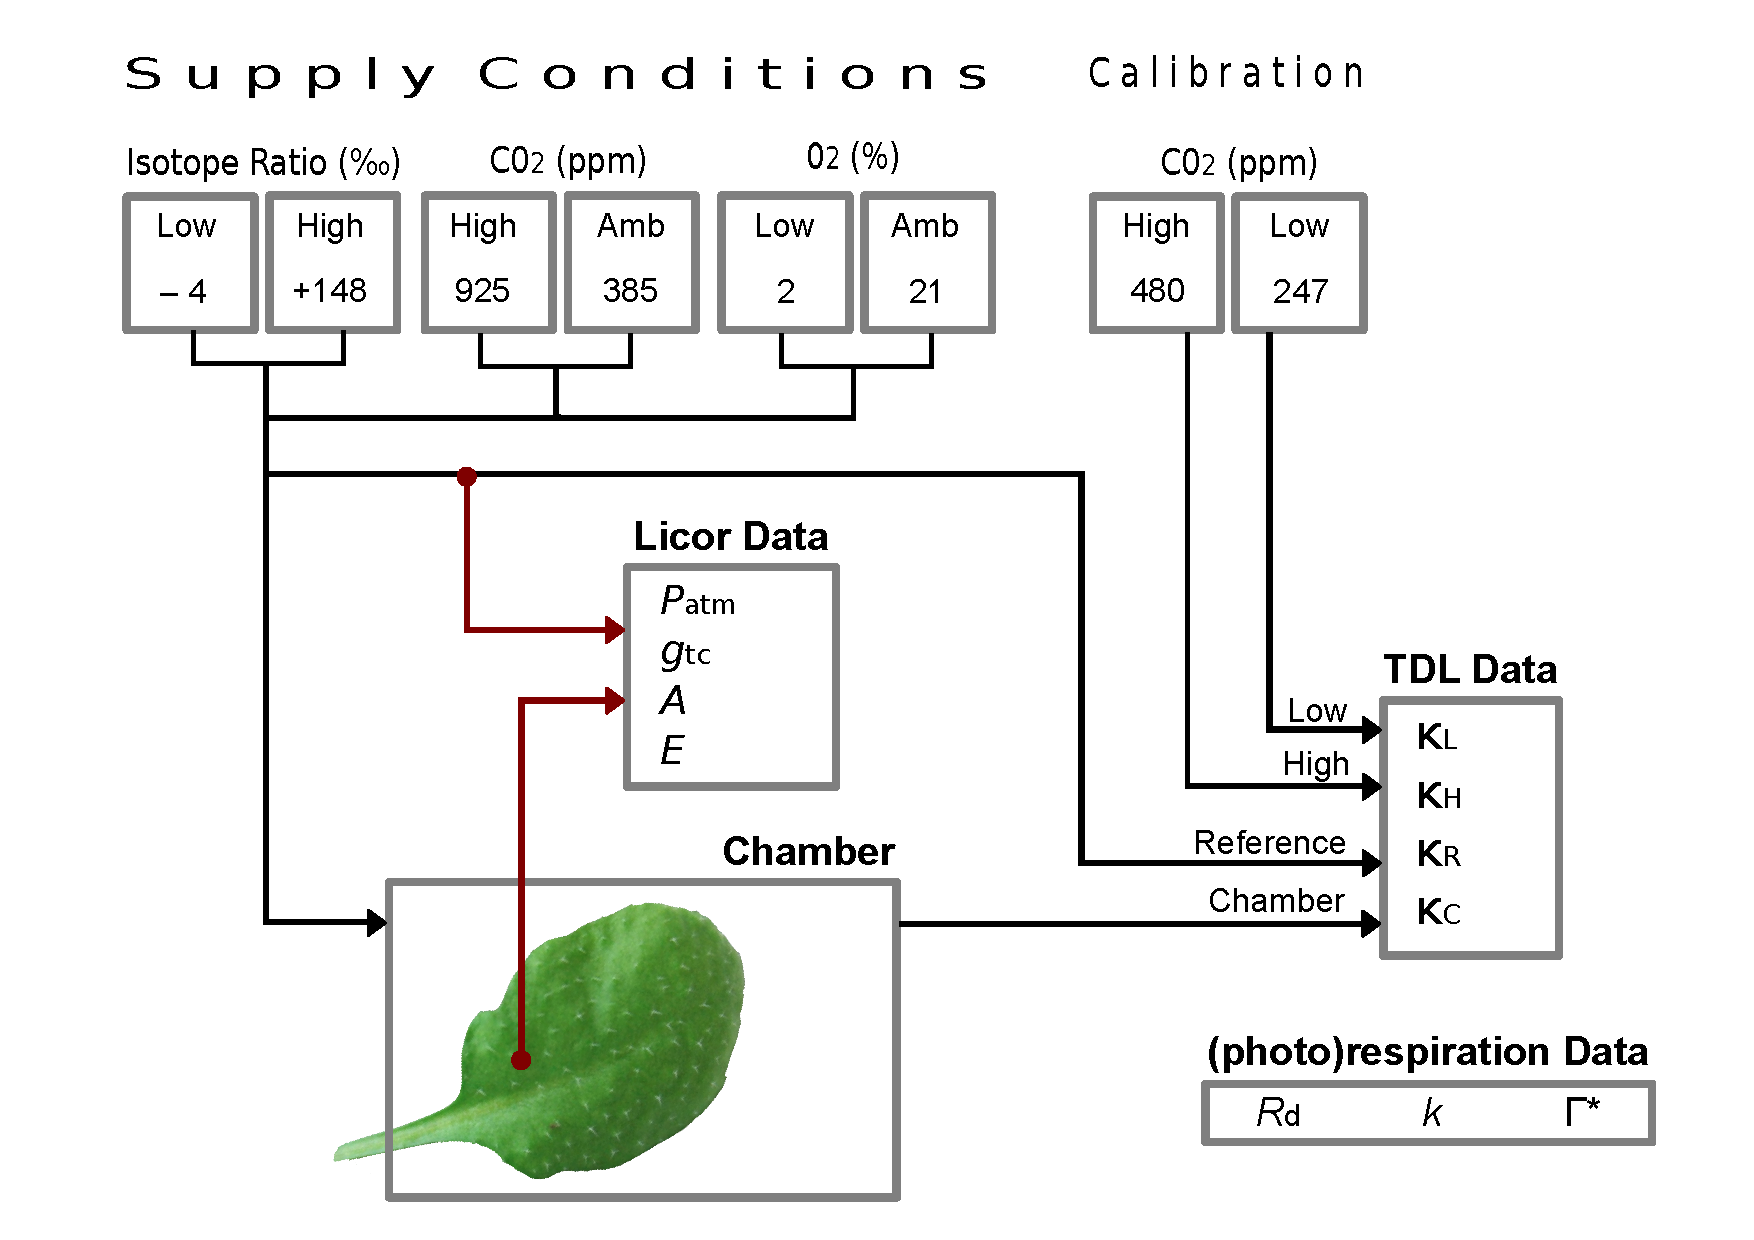
\includegraphics[width=0.8\textwidth]{Schematic_TDL-Licor2}
\caption{
 % (a)  Modify image to include CO$_2$ leaving the leaf.
  Schematic of the experimental configuration.
  }
\label{fi:tdl}
\end{center}
 \end{figure}

 \begin{table}[!hbtp]
  \begin{center}
\begin{tabular}{rrrrrrll}
\hline
     &          &             &           & \multicolumn{2}{c}{Type ($t=1,2$)} \\
Cond & $\delta$ & CO$_2$      & O$_2$     &  WT  & PMDH & Purpose     & Estimate \\
\hline
$c=3$&   $+148$ & Hi(1000ppm) & Amb(21\%) & 3    & 3 & reduced $\ssf$ & $\lambda$: $(1-\lambda)\ssf$\\
   4 &   $  -4$ & Hi(1000ppm) & Amb(21\%) & 3    & 3 & reduced $\ssf$ & $\lambda$: $(1-\lambda)\ssf$\\
   5 &   $+148$ & Amb(400ppm) & Amb(21\%) & 3    & 3 & baseline       & $\ssf+\sse$\\
   6 &   $  -4$ & Amb(400ppm) & Amb(21\%) & 3    & 3 & baseline       & $\ssf+\sse$\\
   7 &   $+148$ & Amb(400ppm) & Low( 2\%) & 3    & 3 & $\ssf\equiv 0$ & $\sse$\\
   8 &   $  -4$ & Amb(400ppm) & Low( 2\%) & 3    & 3 & $\ssf\equiv 0$ & $\sse$\\
\hline
\end{tabular}
\caption{{\bf Experiment.}  For each of 6 conditions and 2 genotypes, 3 plants are measured.}
\label{tab:design}
\end{center}
 \end{table}



%%%%%%%%%%%%%%%%%%%%%%%%%%%%%%%%%%%%%%%%
\subsection{Comprehensive model for discrimination}

Farquhar's comprehensive model for discrimination \eqref{eq:comp}
  includes terms for respiration $\sse$ and photorespiration $\ssf$ \citep{farquhar1982stomatal,farquhar1984isotopic}.
By conducting controlled experiments that
  precisely estimate the other model parameters
  and that isolate when respiration and photorespiration are active
  we can make inference on $\sse$ and $\ssf$.
 %===============
\begin{eqnarray}
  \sDeltacomp
    & = &
  \spa^{-1}
    \big\lbrack
      \sdotab(\spa-\sps)+\sdota(\sps-\spi)+(\sdotbs+\sdotaw)(\spi-\spc) + \sdotb\spc
\nonumber\\ %===
    &&
    \qquad
      -
      \left\lbrace
        \sse\sRd\ssk^{-1} + \ssf\sGammastar
      \right\rbrace
    \big\rbrack
\label{eq:comp}
\end{eqnarray}
 %===============
Frequentist (bootstrap) methods solve for and estimate an approximate sampling distribution for
  the (photo)respiration parameters by drawing samples from the
  estimated sampling distributions of the other parameters.
The Bayesian approach estimates the posterior joint probability density function (pdf)
  of all these parameters
  conditional on data and prior information
  providing inference for all parameters.

\subparagraph{Illustration of bootstrap method}
To understand the intuition behind the bootstrap method,
  let's see how to estimate an intermediate pressure parameter, $\spa$.
The basic structure is that each parameter depends on a combination of
  constants (fixed and assumed known),
  sampling distributions of parameter estimates informed by data,
  or other parameters.
Thus, all parameters are ultimately informed by constants or data.

First we define notation.
Let ``dot'', $\dot{x}$, indicate a constant,
  ``tilde'', $\data{x}$, indicate data, and
  ``undertilde'', $\vector{x}$, indicate a vector.
The four subscripts are
  $c$=condition (1, 2, 3, 4, 5, 6; Table~\ref{tab:design}),
  $t$=genotype (1=WT, 2=PMDH),
  $p$=plant number (1, 2, 3), and
  $r$=repetition (1, 2, 3).

This pressure term,
  $\spa = (\sCa 10^{-6})(\spatmL 10^3)$,
  depends on a concentration ($\sCa$) and the atmospheric pressure ($\spatmL$).
The atmospheric pressure from is measured from the Licor instument,
  and we assume that the observed data follow a normal distribution
  for which we estimate the mean and variance from the sample data,
    $\sdatapatmL \sim \Normal(\spatmL,\ssigpatmL)$.
The concentration of CO$_2$ in the chamber depends on
  the corrected concentration of $^{12}$C and $^{13}$C and a constant,
  $\sCa \equiv \sCo = (\skappaCtwp+\skappaCthp)(1-\sdotfthC)^{-1}$.
The constant is the fraction of C isotopologues not measured, $\sdotfthC\equiv 0.004922$.
The corrected concentrations depend on the observed concentrations,
  as well as calibration gain and offset values,
  $\skappaCtwp = \skappaCtw\sgtw + \sotw$ and
  $\skappaCthp = \skappaCth\sgth + \soth$.
The offset depends on constatnts, the gain, and the observed concentrations.
The known concentration constants for high and low calibration tanks are
  $\vdotkappaHtw
    \equiv (\sdotkappaHtw, \sdotkappaHth)^\transpose
    \equiv (473.3358029, 5.183209292)^\transpose      $ and
  $\vdotkappaLtw
    \equiv (\sdotkappaLtw, \sdotkappaLth)^\transpose
    \equiv (243.4737846, 2.666301131)^\transpose      $.
The gain depends on constants and observed concentrations,
  $\sgtw = (\sdotkappaHtw - \sdotkappaLtw)(\skappaHtw - \skappaLtw)^{-1}$ and
  $\sgth = (\sdotkappaHth - \sdotkappaLth)(\skappaHth - \skappaLth)^{-1}$.
Finally, we assume that the observed concentrations follow a bivariate normal distribution
  for which we estimate the mean and covariance from the sample data,
  $\vdatakappaH \sim \Normal(\vkappaH,\vsigkappaH)$ and
  $\vdatakappaL \sim \Normal(\vkappaL,\vsigkappaL)$.

Each parameter has a similar chain of dependencies.
The bootstrap draws samples from the sampling distributions
  and the series of parameter relationships are used to make inference
  on parameters of interest, including the uncertainty associated with all other parameters.


The posterior joint pdf of all these parameters
  conditional on data and priors
  provides inference for all parameters.

While $\sDeltacomp$ is intended for making predictions,
  in the current experiment it estimates what is observed,
  $\sDeltaobs$.
Therefore, we set $\sDeltacomp\equiv\sDeltaobs$.

%%%%%%%%%%%%%%%%%%%%
\subsubsection{Respiration and photorespiration}

For simplicity, let the pressure terms be
 %===============
\begin{eqnarray}
  \sallpressures
    & \equiv &
  \sdotab(\spa-\sps)+\sdota(\sps-\spi)+(\sdotbs+\sdotaw)(\spi-\spc) + \sdotb\spc.
\nonumber
\end{eqnarray}
 %===============

The comprehensive model may be written as
 %===============
\begin{eqnarray}
  \spa\sDeltaobs
    & = &
  \sallpressures - ( \sse\sRd\ssk^{-1} + \ssf\sGammastar ).
\nonumber
\end{eqnarray}
 %===============

Solving for $\sse$ and $\ssf$, we obtain
 %===============
\begin{eqnarray}
  \sseprime
    & = &
  (\sallpressures - \spa\sDeltaobs - \ssf\sGammastar )(\sRd\ssk^{-1})^{-1}
\nonumber\\ %===
  \ssfprime
    & = &
  (\sallpressures - \spa\sDeltaobs - \sse\sRd\ssk^{-1} )(\sGammastar)^{-1}
\nonumber
\end{eqnarray}
 %===============
where we let our observed values each be distributed normally:
 %===============
\begin{eqnarray}
  \sseprime
    & \sim &
  \Normal(\sse,\sdatasig{\sse}) \quad\textrm{and}
\nonumber\\ %===
  \ssfprime
    & \sim &
  \Normal(\ssf,\sdatasig{\ssf}).
\nonumber
\end{eqnarray}
 %===============
{\bf (priors for e and f)}

These (photo)respiration parameters are currently estimated in another way {\bf (why)},
and are taken as plant-level estimates each with a condition/genotype-specific mean
  and common variance.

Rd is estimated as 0.5 of the dark respiration and assumed to be independent of condition.

$k$ and $\Gamma^{\ast}$ are each estimated from other datasets,
  so we take them as input as data to this model.

 %===============
\begin{eqnarray}
  \sdataRd
    & \sim &
  \Normal(\sRd,\ssigRd)
\nonumber\\ %===
  \sdatak
    & \sim &
  \Normal(\ssk,\ssigk)
\nonumber\\ %===
  \sdataGammastar
    & \sim &
  \Normal(\sGammastar,\ssigGammastar)
\nonumber
\end{eqnarray}
 %===============



% END

